\documentclass[12pt]{article}
\usepackage[UTF8]{ctex}
\usepackage{pythonhighlight}
\usepackage{markdown}
\usepackage{listings}

\lstset{language=C, %用于设置语言为bash
    keywordstyle=\color{purple}\bfseries, %设置关键词为蓝色,需要引xcolor宏包
    identifierstyle=\color{brown!80!black},
    basicstyle=\small, 
    commentstyle=\it\color[RGB]{100,100,100},%基本和注释的字体都使用默认的等宽,而非texlive调用的中文字体
    showstringspaces=false, %不显示中间的空格
    %frame=trBL,  %边框
    %frame=leftline,topline,rightline, bottomline,
    numbers=left,
    numberstyle=\it
}


% Language setting
% Replace `english' with e.g. `spanish' to change the document language
\usepackage[english]{babel}
\usepackage{float}
% Set page size and margins
% Replace `letterpaper' with `a4paper' for UK/EU standard size
\usepackage[letterpaper,top=2cm,bottom=2cm,left=3cm,right=3cm,marginparwidth=1.75cm]{geometry}

% Useful packages
\usepackage{amsmath}
\usepackage{graphicx}
\usepackage[colorlinks=true, allcolors=blue]{hyperref}

\title{Project3 Hard}


\begin{document}
\maketitle

\begin{abstract}
    The 2nd-shortest Path
\end{abstract}

\section*{Chapter 1:Introduction}
    Given a directed graph,find the second shortest path from the start point to the end point in this directed graph,
output the corresponding path length and the corresponding path line,The second-shortest path is the shortest path whose length is longer than the shortest path(s) ,
if two or more shortest paths exist, the second-shortest path is the one whose length is longer than those but no longer than any other path,
and the second-shortest path can backtrack,so that it can use the same road more than once.
\section*{Chapter 2:Algorithm Specification}

\subsection*{Step1:Store the directed graph}
    In this project,I used adjacency list to store the information of Graph,Compared with the adjacency matrix, it can save more memory space,
The relevant statement is as follows:
\begin{figure}[H]
	\centering
	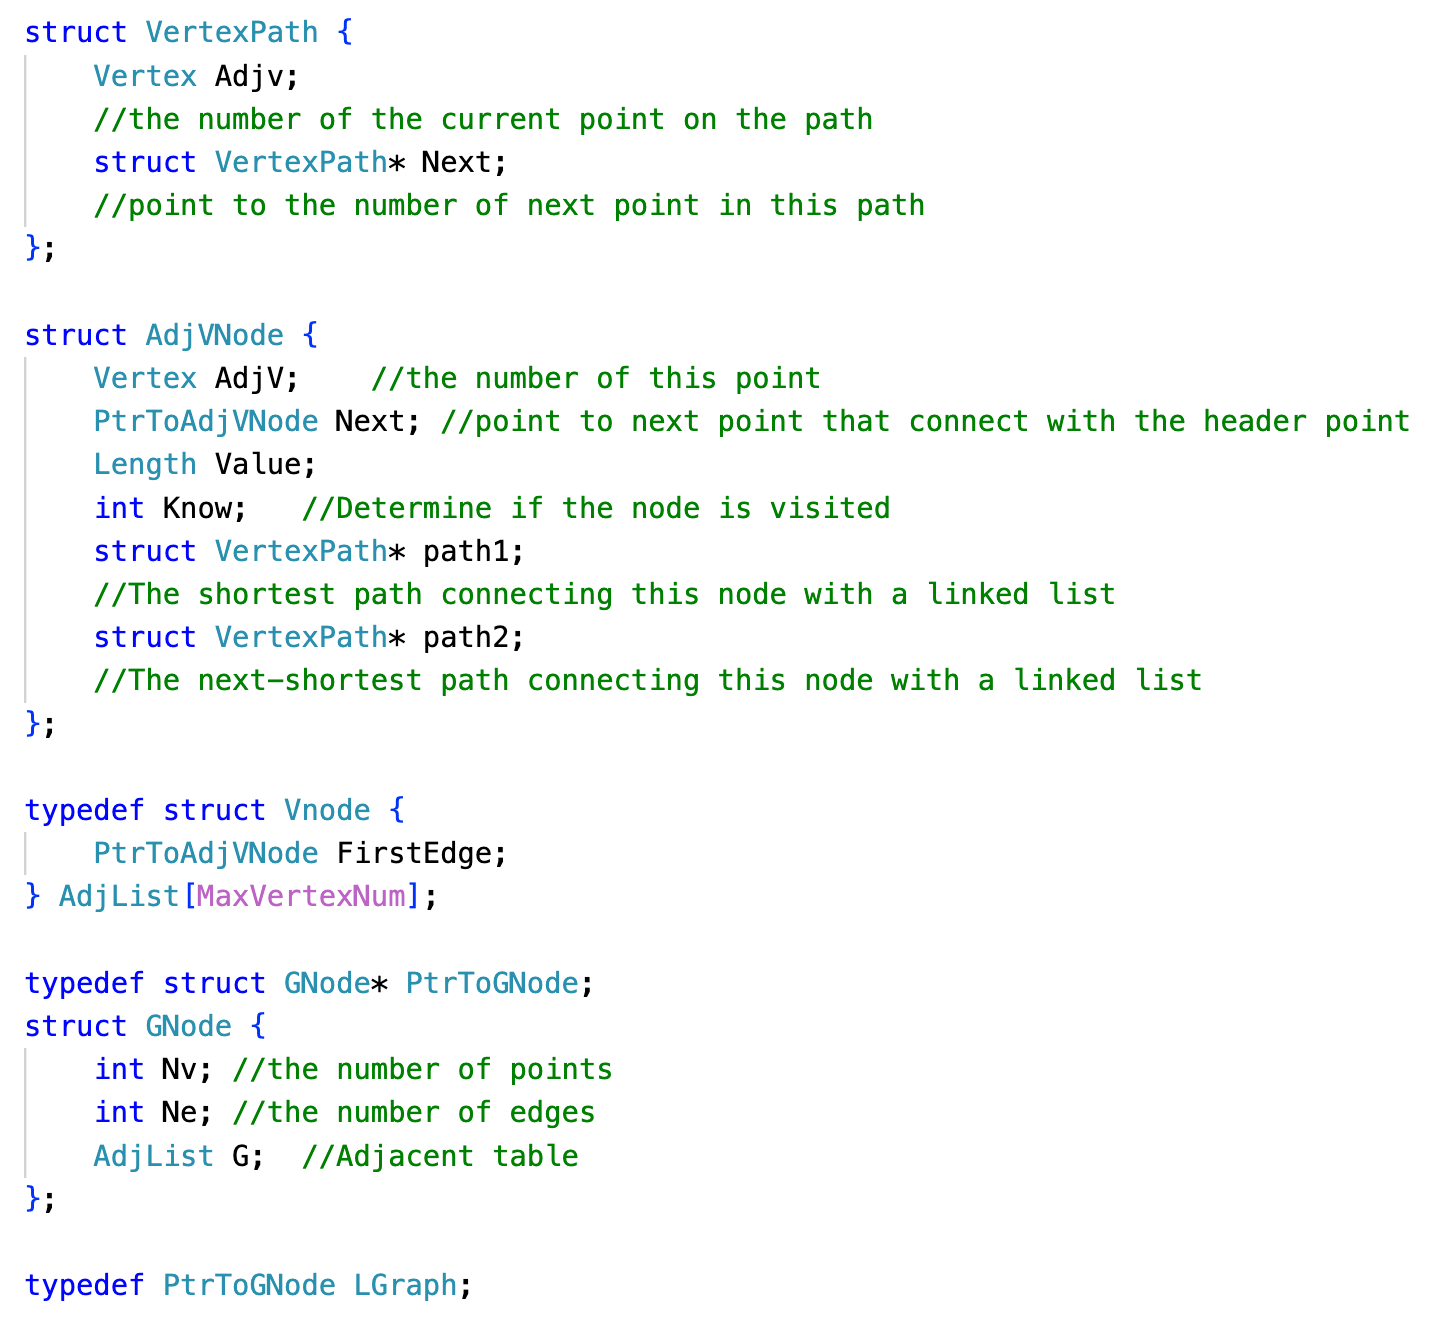
\includegraphics[width=1\textwidth]{1.png}
	\caption{\label{pr}The Declaration for Graph}
	\end{figure}
The meaning of each content has been explained in the notes.

\subsection*{Step2:Find the path}
    In my project i use Dijkstra algorithm's revise to find the second shortest path,we use dist1
to store the shortest path and dist2 to store the second shortest path,Before the algorithm starts, except the dist1 of the starting point, the dist1 and dist2 of the other points are initialized to positive infinity,
in each loop we find the smallest dist1's corresponding node(v1),Traverse its adjacent points,if 

(1):dist1[v1]+value(v1->vk) less than dist1[vk],then changed vk's reference information,
if the old dist1[k] less then the old dist2[k](According to the algorithm, dist2 may be assigned first, but dist1 is still positive and infinite, so this problem should be avoided),
then we changed dist2[k] to dist1[k],and record the path(The change of the path is carried out by the change of the pointer),the changed for dist2[k] will The second shortest path affecting its critical point,then we let k into queue\_dist2[] to change its adjacent points. 
Then we changed the old dist1[k],and and record the path。

(2):dist1[v1]+value(v1->vk) more than dist1[k] but more than dist2[k],then we should change dist2,And it is the same as the method of updating dist2 in (1) 

(3):If the queue\_dist2[] is not empty,then we should get a vertex from it,then  Check and update the adjacent points of this point. If its adjacent points are updated, the changed points must also be enqueued.
In the process of modifying dist2, there is no restriction on whether the point has been visited, so the problem of repeating edges can be solved.

\subsection*{Step3:Use Min-Heap to find dist1}
In order to obtain the smallest dist1 more efficiently,i use the min-heap to store dist1,and adjust the heap every time dist1 is modified.

\subsection*{Step4:Print the Path}
    Because I store the path by a linked list in  'struct VertexPath* path2',then use it we can find the second-shortest path easily.

\section*{Chapter 3:Testing Results}

\subsection*{Test1:}
\begin{figure}[H]
	\centering
	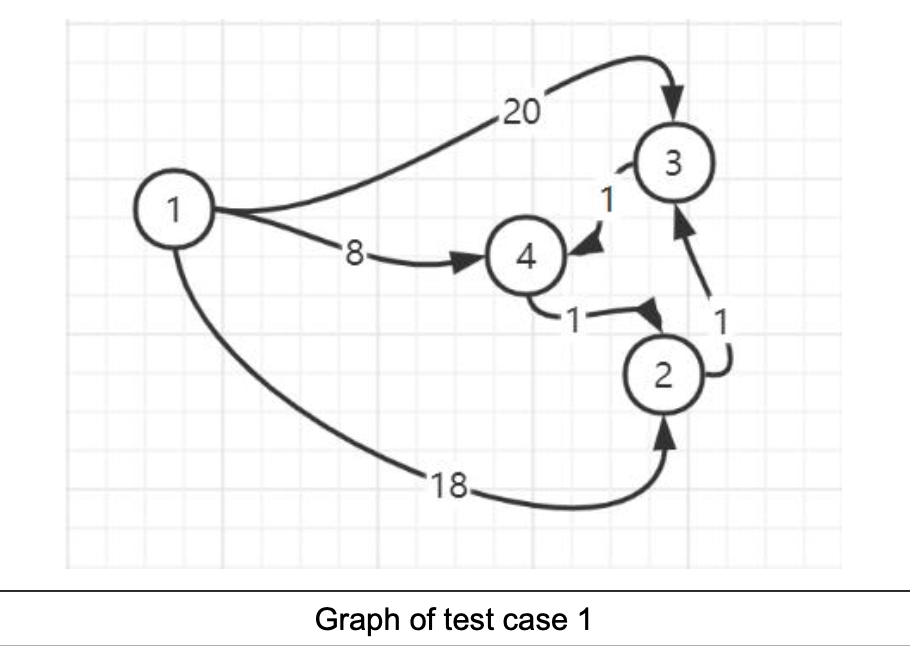
\includegraphics[width=0.7\textwidth]{2.png}
	\caption{\label{pr}test1}
	\end{figure}
The output is:11 1 4 2 3 4

The purpose of this test case is to test the correctness of the algorithm when there exists one small loop in the graph. 
From the graph, we can obviously find that the shortest path from 1 to 4 is 1-4 directly. 
However, when it comes to the second-shortest path, because the path from 1 to 3 and the path from 1 to 2 are too long and the loop 4-2-3-4 is short, 
so the second-shortest path from 1 to 4 is 1-4-2-3-4. 

My program can deal with this situation coreectly.

\subsection*{Test2:}
\begin{figure}[H]
	\centering
	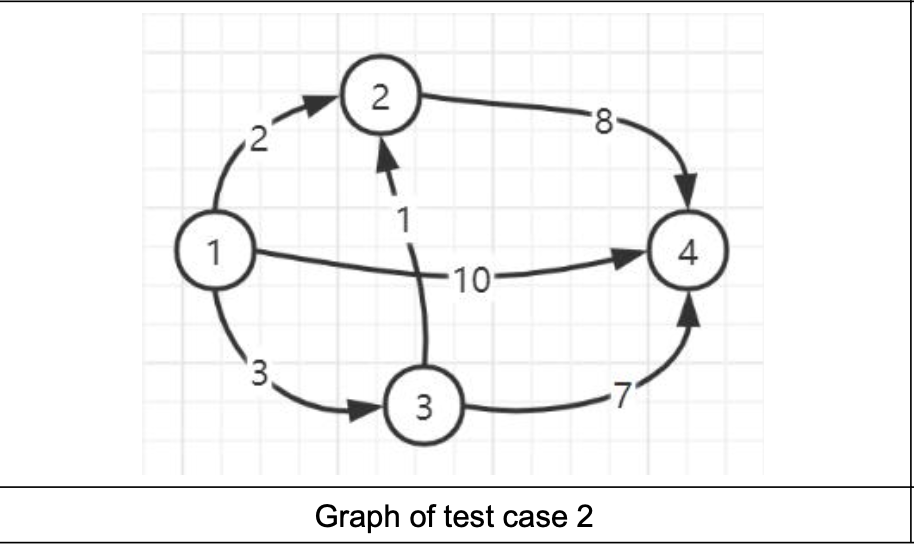
\includegraphics[width=0.7\textwidth]{3.png}
	\caption{\label{pr}test1}
	\end{figure}

The output is:12 1 3 2 4

In this case there are more than one shortest path,from 1 to 4,and my programm find the second-shortest coreectly.

\subsection*{Test3:}
\begin{figure}[H]
	\centering
	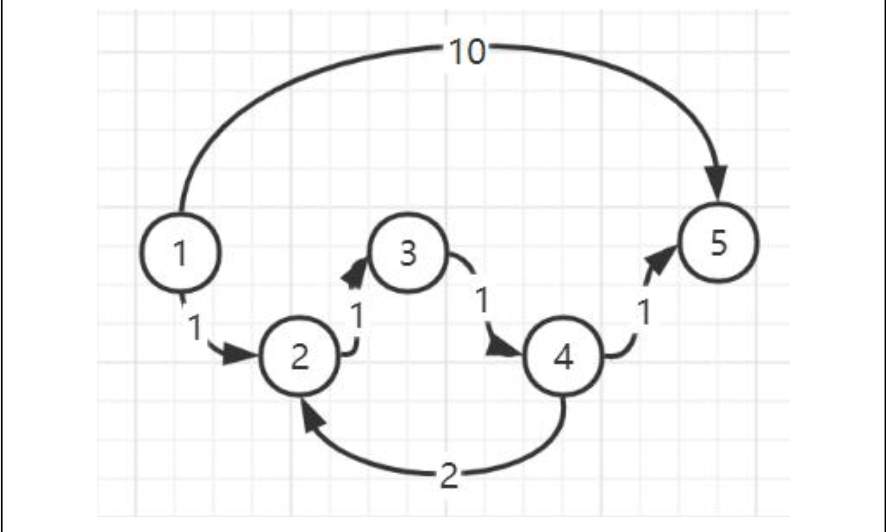
\includegraphics[width=0.7\textwidth]{4.png}
	\caption{\label{pr}test1}
	\end{figure}
The output is:8 1 2 3 4 2 3 4 5

In this case there are 'backtrack' edges in this answer,such as '2->3','3->4', in this case my program can solve it coreectly.

\subsection*{Test4:}
\begin{figure}[H]
	\centering
	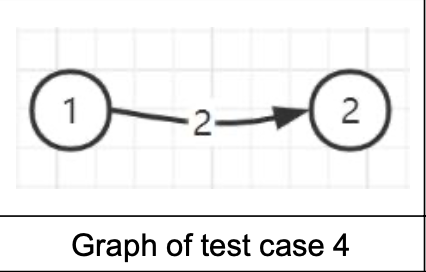
\includegraphics[width=0.7\textwidth]{5.png}
	\caption{\label{pr}test1}
	\end{figure}

The output is:No the second shortest path

In this case there is no the second-shortest path,my program can deal with it coreectly.

\subsection*{Test5:}
\begin{figure}[H]
	\centering
	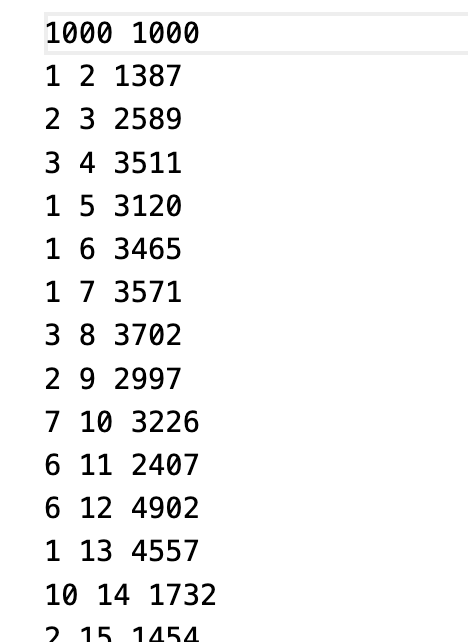
\includegraphics[width=0.4\textwidth]{6.png}
	\caption{\label{pr}test1}
	\end{figure}

The output is:19567 1 6 11 277 531 582 759 993 1000

In this case my program can deal with the problem that has many nodes.

\subsection*{Test6:}
\begin{figure}[H]
	\centering
	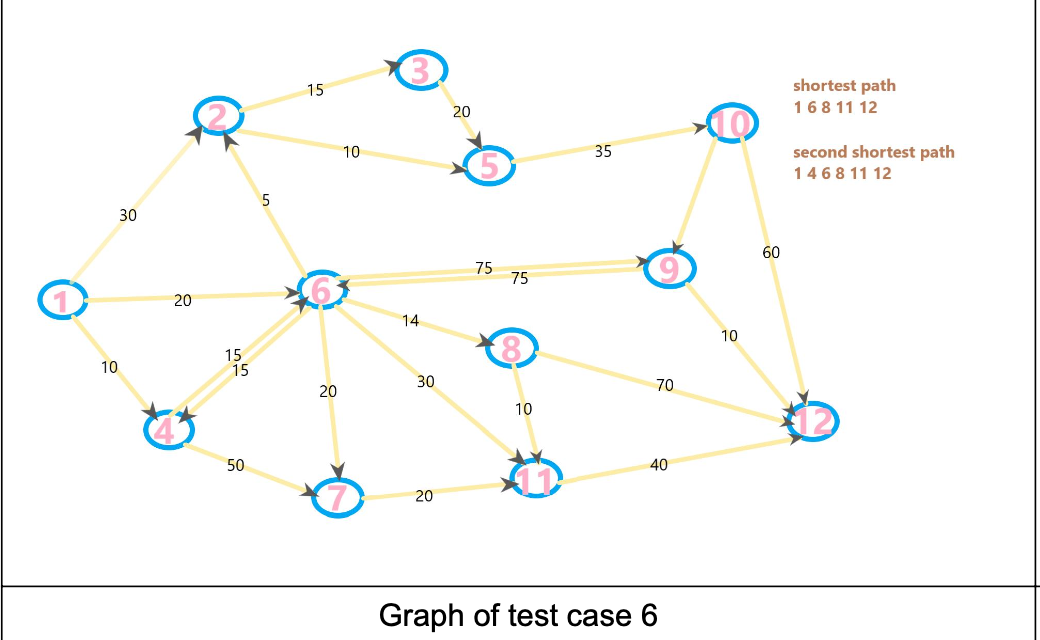
\includegraphics[width=0.4\textwidth]{7.png}
	\caption{\label{pr}test1}
	\end{figure}

The output is:89 1 4 6 8 11 12

In this case there are multiple roads between two vertexs,my programm can deal with it coreectly.

\section*{Chaper 4:Analysis and Comments}

\subsection*{Space Complexity:}
In my project I use Adjacency list to store this Graph,so the Space Complexity is O(V+E).

\subsection*{Time complexity:}

\subsubsection*{The operations of heap:}
To make a heap,because the initialize value of each points except Source are infinite,so we should not do something else,
the time complexity of it is O(1).

The operations of DeleteMin,and Change dist1 is O(logV),Using the method of filtering upwards, this is the basic operation of the heap.


\subsection*{Find the second shortest path:}
The best case: In a best case,if we almost not change dist2 in Dijkstra loop,then we only need to end the program after traversing all the points,
the time complexity is O(V*logV).

The worst case: In a worst case,we should change dist2 for lots of times,when doing a change for dist2,our time complexity is O(V),
and the change for dist2 happens many times,so the time complexity is O($2*V*E + V*logV $).If V >> E,the time complexity 
is O(V*logV),if E >> V, the time complexity is O(V*E).

\subsection*{Print the Path:}
Because i store the path in struct node by pointer path2,so we can get road easily by O(V).

\section*{Appendix:Source (in C)}

You can see the Source code at the end of Report.

\section*{Declaration}
    I hearby declare that all the work done in this project titled"The 2nd-shortest Path"
is of my independent effort.

\end{document}